%!TEX root = main.tex

\section{Dataset and Methodology}
\label{sec:dataset}

We begin this section with the description of packet-level data collection of a mobile voice search service, and then briefly introduce our analysis methodology.

\subsection{Data Collection}

\begin{figure}[th]
	\centering
	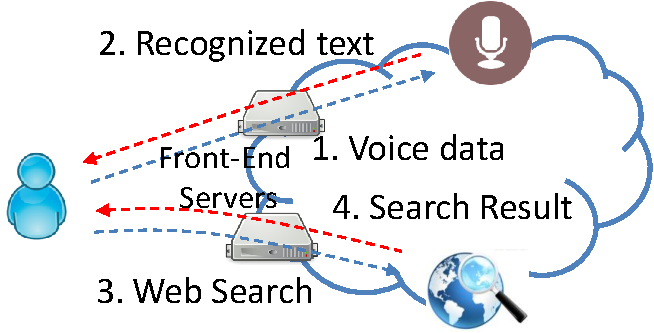
\includegraphics[width=0.8\linewidth]{voice_search_process}
	\caption{Voice search engine infrastructure.}
	\label{fig:voice_search}
\end{figure}

We collect mobile voice search data from Qihoo 360\footnote{http://so.360.cn}, one of the largest service providers in China with market share about 30\% in web search. It serves more than 400 million people per day. A voice search initialized from a mobile terminal consists of two successive phases as shown in Figure~\ref{fig:voice_search}: \emph{voice recognition} (\ie recognize the voice data to query text) and \emph{web search} (i.e. search with returned query text). Voice recognition and web search are served by two types of servers via standard HTTP protocol. As such, a voice search consists of two TCP flows.

%The process of voice search is illustrated in Figure~\ref{fig:voice_search}, which contains two subsequent phases: voice recognition and web search. Mobile client first uploads the voice data and gets the recognized text from voice recognition server, then requests service with the recognized text as the keyword from web search server. The requests in both phases are issued via standard HTTP protocol, in two different TCP flows. 

We collect packet-level traces from front-end servers of both voice recognition and web search, which results in two datasets that correspond to the two phases of voice search. The datasets were collected from March 16th, 2015 to April 19th, 2015, consisting of about 1 million TCP flows.
%The latency between front-end servers and the servers that really serve the requests is below 1~ms, which is negligible in the whole latency that consumers experience. 
All the voice search requests are from mobile apps, especially from Android platform, either via cellular network or WiFi network. The cellular network flows are constituted by a mixture of 2G, 3G and 4G. However, we observed a very limited number of 4G flows in our dataset\footnote{4G network is in the initial deployment in China and has a limited coverage.} and thus omit it from analysis. In total, they make up about 2.5\% of the flows.

Figure~\ref{fig:voice_time_rate} shows the ratio of voice search requests by different access types in a day. The values in the figure are normalized by the maximum value appearing in the dataset. From the figure, the number of requests from both WiFi and cellular network increases from 4 am, and reaches the peak value at 7 pm. The requests of different networks exhibit different access patterns. Clients in 2G/3G network are more likely to request voice search service in the morning before work (from 6 am to 9 am), while clients from WiFi network request more between 6 pm to 9 pm. The different access patterns in different time could guide traffic offloading via request scheduling. 

\begin{figure}[th]
\centering
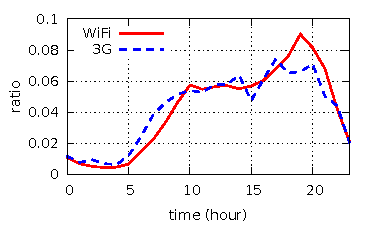
\includegraphics[width=0.8\linewidth]{voice_time_rate}
\caption{The ratio of voice search requests in a day.}
\label{fig:voice_time_rate}
\end{figure}

%The ratio of cellular network flows is about 2.5\%. 

%In the dataset, requests are from three major ISP's in China: China Telecom (CT), China Unicom (CU) and China Mobile (CM). All the three ISP's provide both cellular data network and wireless network accesses. Among the three ISP's, CT provides CDMA (2G) and CDMA2000 (3G), CU provides GPRS (2G) and WCMDA (3G), CM provides GPRS (2G), TD-CDMA (3G) and TD-LTE (4G). The data belonging to 4G occupies a quite small fraction, which could be omitted. The ratio of cellular data flows to all flows is about 2.5\% in all three ISP's.

\subsection{TCP Performance Metrics}

In order to have an in-depth understanding of the performance of voice search, we divide our analysis framework into two parts, corresponding to the two phases of voice search: voice recognition and web search. For a voice search session, both phases contribute to the performance. However, they could have very distinct behavior from the serve-side view. This is because, in the voice recognition phase, server acts as TCP receiver, while in the web search phase, serve is TCP sender. Note that TCP is a sender-driven transmission protocol and its transmission performance is basically affected by the efficiency that sender could handle congestion events, as well as the capability that receiver could receive data.

We examine the TCP performance factors of each phase for individual voice search sessions and their impacts on the flow \emph{finish time}. The finish time of a TCP flow measures the duration from the time when client initiates the connection till the time when the last byte of data is acknowledged. However, as the exact time when client initializes SYN packet is not available from server side, we mark the time when serve received the SYN packet as the start of the duration. It is also noteworthy that since we are interested in the network-related performance, the finish time excludes the time consumed by servers to translate voice data into text. In addition, for the web search phase, we only consider flows carrying search results that are dynamically generated by servers and ignore those corresponding to static content like CSS/JavaScript files.  

%In web search service, there are also other files transmitted in different flows, like CSS/JavaScript file. We only concern the flow carrying web search result, because it is dynamic content, whose transmission performance could not be optimized through local caching.

\begin{figure}[th]
\centering
\begin{subfigure}[b]{0.8\linewidth}
	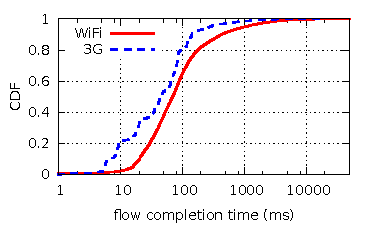
\includegraphics[width=\textwidth]{voice_finish_time}
\caption{Voice recognition}
\label{fig:voice_finish_time}
\end{subfigure} \\
%\vspace{0.1in}
\begin{subfigure}[b]{0.8\linewidth}
	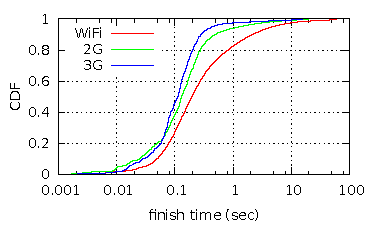
\includegraphics[width=\textwidth]{web_finish_time}
\caption{Web search}
\label{fig:web_finish_time}
\end{subfigure}
\caption{CDFs of finish time in the two phases.}
\label{fig:finish_time}
\end{figure}

%To depict the user-perceived performance in voice recognition and web search, we define performance metric $finish\_time$, measured in seconds. This metric represents the duration from client initiates to establish the connection till the time that the last byte of data is acknowledged.

% Note that mobile client is the sender in voice recognition and is the receiver in web search. In web search service, there are also other files transmitted in different flows, like CSS/JavaScript file. We only concern the flow carrying web search result, because it is dynamic content, whose transmission performance could not be optimized through local caching. As we could not determine the exact time when the SYN packet is transmitted in voice recognition, we use the time when the SYN packet is received to approximate the beginning of the duration, which we will detail later by Figure~\ref{fig:voice_estimate_rtt}.

Figure~\ref{fig:finish_time} plots the cumulative distribution (CDF) of the finish time of TCP flows in the two phases. We surprisingly find that in both phases 2G/3G flows experience a shorter finish time than WiFi flows. Indeed, the 2G and 3G flows show similar performance. Another notable finding is that some flows experience an extraordinarily long finish time compared with others. For example, while most of the voice recognition flows finish in 0.1 second, a non-negligible fraction of flows (5\% in WiFi, and 2\% in 2G/3G) take more than 1 second to upload the voice data. We were motivated by these observations to have an in-depth analysis of the TCP performance and its impact on the flow finish time in mobile voice search.

%From Figure~\ref{fig:voice_finish_time}, the overall finish time of flows in 2G/3G in shorter than that of flows in WiFi network. The median values of finish time in the three access types are 0.069s in WiFi, 0.045s in 2G, and 0.044s in 3G, respectively. We also see that more than a large fraction of of voice recognition flows (60\% in WiFi and 80\% in 2G/3G) experience latency of less than 0.1s. However, a non-negligible fraction of flows (5\% in WiFi, and 2\% in 2G/3G) takes more than 1 second to upload the voice data.

%Figure~\ref{fig:web_finish_time} shows the CDF of finish time of web search flows. In the figure, the overall finish time of flows in 2G and 3G (with median values 0.013s and 0.011s) in also shorter than that of flows in WiFi network (with median value 0.2s). More than 25\% of flows in all networks experience finish time less than 0.1 second. However, 5\% of flows in 2G network and 18\% in WiFi network experience finish time more than 1 second. Furthermore, about 3\% of flows in WiFi network are with finish time more than 10 seconds, which is a great performance degradation.

A comparison of the TCP flow finish time between voice recognition and web search in Figure~\ref{fig:finish_time} shows that the finish time in web search contribute to the majority of the user perceived performance of a voice search session. However, it by no means indicates that understanding the performance of voice recognition flows is not as important as that of web search flows. This is because voice recognition is the first step of the whole voice search process and a long recognition time would certainly result in bad user experience, even early quit of the process.

% some of voice recognition flows suffer from timeout retransmission, which is a great performance degradation~\cite{flach2013reducing}. Second, a non-negligible fraction of voice recognition flows are terminated before voice data transmission completes. These bad user experiences also inspire us to understand what factors and how they impact user-perceived performance in voice recognition flows.

%\begin{figure}[th]
%\centering
%\begin{subfigure}[b]{0.8\linewidth}
%	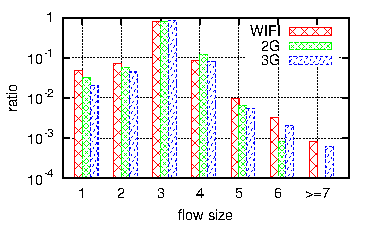
\includegraphics[width=\textwidth]{voice_flow_size}
%\caption{Voice recognition}
%\label{fig:voice_flow_size}
%\end{subfigure} \\
%%\vspace{0.1in}
%\begin{subfigure}[b]{0.8\linewidth}
%	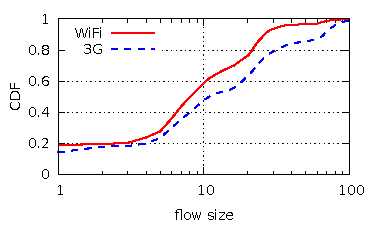
\includegraphics[width=\textwidth]{web_flow_size}
%\caption{Web Search}
%\label{fig:web_flow_size}
%\end{subfigure}
%\caption{The distribution of flow sizes (in packet) in the two phases.}
%\label{fig:flow_size}
%\end{figure}
%
%Next, we investigate the distribution of flow size (in packet) in the two phases, which is shown in Figure~\ref{fig:flow_size}. It is worth noting that flow size does not include the packet carrying text in voice recognition and the HTTP GET packet in web search. Figure~\ref{fig:voice_flow_size} shows the ratio of flows with various sizes, in which the $y$-axis is drawn in log scale. From the figure, nearly all flows contain no more than 6 data packets. Among all access types, about 80\% of voice recognition flows are with 3 data packets. The initial congestion window in current Android TCP/IP stack is set to 10 segments\cite{dukkipati2010argument}, which means the voice data could be transmitted in the initial congestion window.
%
%Figure~\ref{fig:web_flow_size} shows the CDF of flow sizes in web search. From the figure, all flows are with less than 100 data packets, in which a large fraction of flows are with size in range between 4 and 30 packets. There are also flows with no search result, resulting in one data packet in the flow, which occupy 15\% of flows. The median value of flow size in WiFi network is smaller than that of flows in 2G/3G network. This may be induced by different customized designs for different access types.
%
%The flow size in web search ranges from 1 to 100 packets. This means that the data could be transmitted in 1 RTT at least, and more than 4 RTT at most. Considering the various flow sizes, the metric $finish\_time$ could not portray the efficiency that the data is delivered. To eliminate the affect of flow size, we introduce one more performance metric transmission speed ($trans\_speed$), defined as the average time to transmit a data packet. The metric $trans\_speed$ could be represented as $\frac{finish\_time}{\#(pkts)}$.

%To evaluate the impact of network quality on user experience in voice search, we mainly consider the following network factors in the analysis:
In particular, we consider the following TCP performance factors. 

\begin{itemize}
%\setlength{\itemsep}{-8pt}
%\setlength{\topsep}{-8pt}
%	\item {Access Type: } Mobile client could issue the voice search service via 2G/3G/4G or WiFi network. Different access types exhibit different network characteristics. For example, compared with WiFi network, the latency in cellular network is smaller, while packet loss or reordering event is more common. \\
	\item {Round Trip Time (RTT): } RTT is a commonly used indicator of TCP performance, especially for short TCP flows like search flows.
	
%	If two senders have the same congestion window size, the one with smaller RTT will receive acknowledgments in shorter time, thus could transmit more data per unit time, resulting smaller $finish\_time$. \\

	\item {Number of lost/disordered packets: } Both packet loss and packet reordering could affect the transmission efficiency. Packet loss leads to reduction of sender's congestion window. Although packet reordering does not reduce congestion window, it will prevent congestion window from growing and may trigger spurious retransmission. \\
	
	\item {Timeout Retransmission: } This metric is an indicator whether there is a timeout retransmission or not in the flow. Timeout retransmission could be triggered due to insufficient number of duplicate acknowledgments under packet loss~\cite{rfc6675}. The RTO timer could be set to more than 200~ms in current Linux/Android implementation, and will be doubled if the retransmitted packet is dropped, which is exceptionally high in short flows~\cite{flach2013reducing}.\\
	
\end{itemize}

When examining the impact of the above factors on TCP finish time, we also consider the potential impact of TCP flow size and the access type (i.e. 2G, 3G or WiFi). 

%To summarize, we mainly investigate the impact of network factors, including \emph{access type}, \emph{RTT}, \emph{network event}, \emph{timeout retransmission}, on user-perceived performance in voice search process, including $finish\_time$, $trans\_speed$.

%\subsection{Analysis Methodology}
%
%We use both correlation coefficient and QED (Quasi-Experimental Design) to evaluate the impact of TCP performance factors on flow finish time. % a collection of analysis methodologies to determine which factors matter the most, and how much a factor affects the performance quantitatively.
%
%\subsubsection{Correlation}
%
%%Correlation coefficient is the natural approach to depict the interaction between two variables. Here we use Pearson Correlation Coefficient (PCC) to quantify the magnitude of relationship between network factors and performance metrics in voice search service. PCC is a measure of linear correlation between two numeric variable $x$ and $y$. PCC determines the correlation coefficient via formula $\text{corr}(x,y) = \frac{\text{cov}(x,y)}{\text{dev}(x) \text{dev}(y)}$, where $\text{cov}(.,.)$ is the covariance function, and $\text{dev}(.)$ is the standard deviation. The correlation coefficient ranges from -1 to 1, where -1 represents total negative correlation, 0 is no correlation, and -1 is total positive correlation.
%
%We use the Kendall correlation coefficient to measure the correlation between a TCP performance factor and flow finish time. Kendall's correlation is a kind of rank correlation and does not assume any particular distributional relationship between the two variables. The correlation $\tau$ lies in between -1 and 1, where ``1'' means a perfect positive correlation, ``-1'' refers to a perfect negative correlation and ``0'' implies the two variables are independent. In detail, we group the flows into bins with appropriate intervals of the TCP performance factor (i.e. RTT, packet loss/packet reordering, timeout retransmission), and obtain the mean finish time of flows in each bin. We then compute the Kendall correlation coefficient between bin indices and the mean finish time values. We use the binned indices instead of directly computation of the correlation for two reasons. First, our goal is to characterize a general trend of the correlation between performance factors and finish time, and the binned data can eliminate the noise in data. The second reason is related to the computation time. Computing the rank correlation of millions flows is indeed computationally expensive. 

%\subsubsection{Quasi-Experimental Design (QED)}
%
%%To casually depict the impact of network factors on user-perceived performance, we adopt controlled experiment methodology ``Quasi-Experimental Design'' (QED) \cite{krishnan2013video}. The basic idea of QED is to investigate the significance of a factor $x$ by varying this factor while controlling other factors as invariable.
%
%In order to further investigate the correlation between TCP performance factor and flow finish time, we implement a non-parametric factorial analysis framework using a Quasi Experimental Design (QED) \cite{krishnan2013video}. This approach is used to assess the objective impact of a cause variable on an outcome variable by excluding the possible effect of other covariates. In QED, each uniformly sampled individual $u$ is compared with an individual $v$ randomly selected from those that have identical covariates with $u$ but the cause variable. And thus, any outcome difference between these two individuals can be attributed to the cause variable we are tracking. 
%
%The QED analysis is best illustrated with the following example. Suppose we aim at understanding the impact of packet loss event on finish time. Flows are first grouped into bins $\{ F_0, F_1, F_2, \cdots, F_n \}$ according the number of lost packets, where the index is the number of lost packets. We take $F_0$ (\ie with no lost packet) as the baseline. For each flow $u$ in $F_0$, we randomly choose a flow $v$ in $F_i$, having similar properties to flow $u$: access type, RTT, flow size and timeout retransmission. We record the outcome difference as $o_{u,v} = finish\_time_{v} / finish\_time_{u}$. Finally, we average all the outcome differences over the matched pairs and use this average difference to gauge the impact of losing $i$ packets.

